% REV01 Sun 27 Jun 2021 14:11:59 WIB
% START Tue 04 May 2021 13:55:16 WIB

\chapter{SHOWING HOW THE GOLDEN DUSTMAN HELPED TO SCATTER DUST}

In all the first bewilderment of her wonder, the most bewilderingly
wonderful thing to Bella was the shining countenance of Mr Boffin. That
his wife should be joyous, open-hearted, and genial, or that her face
should express every quality that was large and trusting, and no quality
that was little or mean, was accordant with Bella’s experience. But,
that he, with a perfectly beneficent air and a plump rosy face, should
be standing there, looking at her and John, like some jovial good
spirit, was marvellous. For, how had he looked when she last saw him in
that very room (it was the room in which she had given him that piece of
her mind at parting), and what had become of all those crooked lines of
suspicion, avarice, and distrust, that twisted his visage then?

Mrs Boffin seated Bella on the large ottoman, and seated herself beside
her, and John her husband seated himself on the other side of her, and
Mr Boffin stood beaming at every one and everything he could see, with
surpassing jollity and enjoyment. Mrs Boffin was then taken with a
laughing fit of clapping her hands, and clapping her knees, and rocking
herself to and fro, and then with another laughing fit of embracing
Bella, and rocking her to and fro--both fits, of considerable duration.

‘Old lady, old lady,’ said Mr Boffin, at length; ‘if you don’t begin
somebody else must.’

‘I’m a going to begin, Noddy, my dear,’ returned Mrs Boffin. ‘Only it
isn’t easy for a person to know where to begin, when a person is in this
state of delight and happiness. Bella, my dear. Tell me, who’s this?’

‘Who is this?’ repeated Bella. ‘My husband.’

‘Ah! But tell me his name, deary!’ cried Mrs Boffin.

‘Rokesmith.’

‘No, it ain’t!’ cried Mrs Boffin, clapping her hands, and shaking her
head. ‘Not a bit of it.’

‘Handford then,’ suggested Bella.

‘No, it ain’t!’ cried Mrs Boffin, again clapping her hands and shaking
her head. ‘Not a bit of it.’

‘At least, his name is John, I suppose?’ said Bella.

‘Ah! I should think so, deary!’ cried Mrs Boffin. ‘I should hope so!
Many and many is the time I have called him by his name of John. But
what’s his other name, his true other name? Give a guess, my pretty!’

‘I can’t guess,’ said Bella, turning her pale face from one to another.

‘I could,’ cried Mrs Boffin, ‘and what’s more, I did! I found him out,
all in a flash as I may say, one night. Didn’t I, Noddy?’

‘Ay! That the old lady did!’ said Mr Boffin, with stout pride in the
circumstance.

‘Harkee to me, deary,’ pursued Mrs Boffin, taking Bella’s hands between
her own, and gently beating on them from time to time. ‘It was after a
particular night when John had been disappointed--as he thought--in
his affections. It was after a night when John had made an offer to a
certain young lady, and the certain young lady had refused it. It was
after a particular night, when he felt himself cast-away-like, and had
made up his mind to go seek his fortune. It was the very next night. My
Noddy wanted a paper out of his Secretary’s room, and I says to Noddy,
“I am going by the door, and I’ll ask him for it.” I tapped at his door,
and he didn’t hear me. I looked in, and saw him a sitting lonely by his
fire, brooding over it. He chanced to look up with a pleased kind of
smile in my company when he saw me, and then in a single moment every
grain of the gunpowder that had been lying sprinkled thick about him
ever since I first set eyes upon him as a man at the Bower, took fire!
Too many a time had I seen him sitting lonely, when he was a poor child,
to be pitied, heart and hand! Too many a time had I seen him in need of
being brightened up with a comforting word! Too many and too many a time
to be mistaken, when that glimpse of him come at last! No, no! I just
makes out to cry, “I know you now! You’re John!” And he catches me as
I drops.--So what,’ says Mrs Boffin, breaking off in the rush of her
speech to smile most radiantly, ‘might you think by this time that your
husband’s name was, dear?’

‘Not,’ returned Bella, with quivering lips; ‘not Harmon? That’s not
possible?’

‘Don’t tremble. Why not possible, deary, when so many things are
possible?’ demanded Mrs Boffin, in a soothing tone.

‘He was killed,’ gasped Bella.

‘Thought to be,’ said Mrs Boffin. ‘But if ever John Harmon drew the
breath of life on earth, that is certainly John Harmon’s arm round your
waist now, my pretty. If ever John Harmon had a wife on earth, that wife
is certainly you. If ever John Harmon and his wife had a child on earth,
that child is certainly this.’

By a master-stroke of secret arrangement, the inexhaustible baby here
appeared at the door, suspended in mid-air by invisible agency. Mrs
Boffin, plunging at it, brought it to Bella’s lap, where both Mrs and Mr
Boffin (as the saying is) ‘took it out of’ the Inexhaustible in a shower
of caresses. It was only this timely appearance that kept Bella from
swooning. This, and her husband’s earnestness in explaining further to
her how it had come to pass that he had been supposed to be slain, and
had even been suspected of his own murder; also, how he had put a pious
fraud upon her which had preyed upon his mind, as the time for its
disclosure approached, lest she might not make full allowance for
the object with which it had originated, and in which it had fully
developed.

‘But bless ye, my beauty!’ cried Mrs Boffin, taking him up short at this
point, with another hearty clap of her hands. ‘It wasn’t John only that
was in it. We was all of us in it.’

‘I don’t,’ said Bella, looking vacantly from one to another, ‘yet
understand--’

‘Of course you don’t, my deary,’ exclaimed Mrs Boffin. ‘How can you till
you’re told! So now I am a going to tell you. So you put your two hands
between my two hands again,’ cried the comfortable creature, embracing
her, ‘with that blessed little picter lying on your lap, and you shall
be told all the story. Now, I’m a going to tell the story. Once, twice,
three times, and the horses is off. Here they go! When I cries out that
night, “I know you now, you’re John!”--which was my exact words; wasn’t
they, John?’

‘Your exact words,’ said John, laying his hand on hers.

‘That’s a very good arrangement,’ cried Mrs Boffin. ‘Keep it there,
John. And as we was all of us in it, Noddy you come and lay yours a top
of his, and we won’t break the pile till the story’s done.’

Mr Boffin hitched up a chair, and added his broad brown right hand to
the heap.

‘That’s capital!’ said Mrs Boffin, giving it a kiss. ‘Seems quite a
family building; don’t it? But the horses is off. Well! When I cries
out that night, “I know you now! you’re John!” John catches of me, it
is true; but I ain’t a light weight, bless ye, and he’s forced to let me
down. Noddy, he hears a noise, and in he trots, and as soon as I anyways
comes to myself I calls to him, “Noddy, well I might say as I did say,
that night at the Bower, for the Lord be thankful this is John!” On
which he gives a heave, and down he goes likewise, with his head under
the writing-table. This brings me round comfortable, and that brings him
round comfortable, and then John and him and me we all fall a crying for
joy.’

‘Yes! They cry for joy, my darling,’ her husband struck in. ‘You
understand? These two, whom I come to life to disappoint and dispossess,
cry for joy!’

Bella looked at him confusedly, and looked again at Mrs Boffin’s radiant
face.

‘That’s right, my dear, don’t you mind him,’ said Mrs Boffin, ‘stick
to me. Well! Then we sits down, gradually gets cool, and holds a
confabulation. John, he tells us how he is despairing in his mind on
accounts of a certain fair young person, and how, if I hadn’t found him
out, he was going away to seek his fortune far and wide, and had fully
meant never to come to life, but to leave the property as our wrongful
inheritance for ever and a day. At which you never see a man so
frightened as my Noddy was. For to think that he should have come into
the property wrongful, however innocent, and--more than that--might have
gone on keeping it to his dying day, turned him whiter than chalk.’

‘And you too,’ said Mr Boffin.

‘Don’t you mind him, neither, my deary,’ resumed Mrs Boffin; ‘stick
to me. This brings up a confabulation regarding the certain fair young
person; when Noddy he gives it as his opinion that she is a deary
creetur. “She may be a leetle spoilt, and nat’rally spoilt,” he says,
“by circumstances, but that’s only the surface, and I lay my life,” he
says, “that she’s the true golden gold at heart.”’

‘So did you,’ said Mr Boffin.

‘Don’t you mind him a single morsel, my dear,’ proceeded Mrs Boffin,
‘but stick to me. Then says John, O, if he could but prove so! Then we
both of us ups and says, that minute, “Prove so!”’

With a start, Bella directed a hurried glance towards Mr Boffin. But,
he was sitting thoughtfully smiling at that broad brown hand of his, and
either didn’t see it, or would take no notice of it.

‘“Prove it, John!” we says,’ repeated Mrs Boffin. ‘“Prove it and
overcome your doubts with triumph, and be happy for the first time in
your life, and for the rest of your life.” This puts John in a state,
to be sure. Then we says, “What will content you? If she was to stand up
for you when you was slighted, if she was to show herself of a generous
mind when you was oppressed, if she was to be truest to you when you was
poorest and friendliest, and all this against her own seeming interest,
how would that do?” “Do?” says John, “it would raise me to the skies.”
 “Then,” says my Noddy, “make your preparations for the ascent, John, it
being my firm belief that up you go!”’

Bella caught Mr Boffin’s twinkling eye for half an instant; but he got
it away from her, and restored it to his broad brown hand.

‘From the first, you was always a special favourite of Noddy’s,’ said
Mrs Boffin, shaking her head. ‘O you were! And if I had been inclined
to be jealous, I don’t know what I mightn’t have done to you. But as I
wasn’t--why, my beauty,’ with a hearty laugh and an embrace, ‘I made you
a special favourite of my own too. But the horses is coming round the
corner. Well! Then says my Noddy, shaking his sides till he was fit to
make ‘em ache again: “Look out for being slighted and oppressed, John,
for if ever a man had a hard master, you shall find me from this present
time to be such to you.” And then he began!’ cried Mrs Boffin, in an
ecstacy of admiration. ‘Lord bless you, then he began! And how he DID
begin; didn’t he!’

Bella looked half frightened, and yet half laughed.

‘But, bless you,’ pursued Mrs Boffin, ‘if you could have seen him of a
night, at that time of it! The way he’d sit and chuckle over himself!
The way he’d say “I’ve been a regular brown bear to-day,” and take
himself in his arms and hug himself at the thoughts of the brute he had
pretended. But every night he says to me: “Better and better, old lady.
What did we say of her? She’ll come through it, the true golden gold.
This’ll be the happiest piece of work we ever done.” And then he’d say,
“I’ll be a grislier old growler to-morrow!” and laugh, he would, till
John and me was often forced to slap his back, and bring it out of his
windpipes with a little water.’

Mr Boffin, with his face bent over his heavy hand, made no sound,
but rolled his shoulders when thus referred to, as if he were vastly
enjoying himself.

‘And so, my good and pretty,’ pursued Mrs Boffin, ‘you was married, and
there was we hid up in the church-organ by this husband of yours; for
he wouldn’t let us out with it then, as was first meant. “No,” he says,
“she’s so unselfish and contented, that I can’t afford to be rich yet. I
must wait a little longer.” Then, when baby was expected, he says, “She
is such a cheerful, glorious housewife that I can’t afford to be rich
yet. I must wait a little longer.” Then when baby was born, he says,
“She is so much better than she ever was, that I can’t afford to be rich
yet. I must wait a little longer.” And so he goes on and on, till I says
outright, “Now, John, if you don’t fix a time for setting her up in her
own house and home, and letting us walk out of it, I’ll turn Informer.”
 Then he says he’ll only wait to triumph beyond what we ever thought
possible, and to show her to us better than even we ever supposed; and
he says, “She shall see me under suspicion of having murdered myself,
and YOU shall see how trusting and how true she’ll be.” Well! Noddy and
me agreed to that, and he was right, and here you are, and the horses is
in, and the story is done, and God bless you my Beauty, and God bless us
all!’

The pile of hands dispersed, and Bella and Mrs Boffin took a good long
hug of one another: to the apparent peril of the inexhaustible baby,
lying staring in Bella’s lap.

‘But IS the story done?’ said Bella, pondering. ‘Is there no more of
it?’

‘What more of it should there be, deary?’ returned Mrs Boffin, full of
glee.

‘Are you sure you have left nothing out of it?’ asked Bella.

‘I don’t think I have,’ said Mrs Boffin, archly.

‘John dear,’ said Bella, ‘you’re a good nurse; will you please hold
baby?’ Having deposited the Inexhaustible in his arms with those words,
Bella looked hard at Mr Boffin, who had moved to a table where he was
leaning his head upon his hand with his face turned away, and, quietly
settling herself on her knees at his side, and drawing one arm over his
shoulder, said: ‘Please I beg your pardon, and I made a small mistake of
a word when I took leave of you last. Please I think you are better (not
worse) than Hopkins, better (not worse) than Dancer, better (not worse)
than Blackberry Jones, better (not worse) than any of them! Please
something more!’ cried Bella, with an exultant ringing laugh as she
struggled with him and forced him to turn his delighted face to hers.
‘Please I have found out something not yet mentioned. Please I don’t
believe you are a hard-hearted miser at all, and please I don’t believe
you ever for one single minute were!’

At this, Mrs Boffin fairly screamed with rapture, and sat beating her
feet upon the floor, clapping her hands, and bobbing herself backwards
and forwards, like a demented member of some Mandarin’s family.

‘O, I understand you now, sir!’ cried Bella. ‘I want neither you nor any
one else to tell me the rest of the story. I can tell it to YOU, now, if
you would like to hear it.’

‘Can you, my dear?’ said Mr Boffin. ‘Tell it then.’

‘What?’ cried Bella, holding him prisoner by the coat with both hands.
‘When you saw what a greedy little wretch you were the patron of, you
determined to show her how much misused and misprized riches could
do, and often had done, to spoil people; did you? Not caring what she
thought of you (and Goodness knows THAT was of no consequence!) you
showed her, in yourself, the most detestable sides of wealth, saying in
your own mind, “This shallow creature would never work the truth out of
her own weak soul, if she had a hundred years to do it in; but a glaring
instance kept before her may open even her eyes and set her thinking.”
 That was what you said to yourself, was it, sir?’

‘I never said anything of the sort,’ Mr Boffin declared in a state of
the highest enjoyment.

‘Then you ought to have said it, sir,’ returned Bella, giving him two
pulls and one kiss, ‘for you must have thought and meant it. You saw
that good fortune was turning my stupid head and hardening my silly
heart--was making me grasping, calculating, insolent, insufferable--and
you took the pains to be the dearest and kindest fingerpost that ever
was set up anywhere, pointing out the road that I was taking and the end
it led to. Confess instantly!’

‘John,’ said Mr Boffin, one broad piece of sunshine from head to foot,
‘I wish you’d help me out of this.’

‘You can’t be heard by counsel, sir,’ returned Bella. ‘You must speak
for yourself. Confess instantly!’

‘Well, my dear,’ said Mr Boffin, ‘the truth is, that when we did go in
for the little scheme that my old lady has pinted out, I did put it to
John, what did he think of going in for some such general scheme as YOU
have pinted out? But I didn’t in any way so word it, because I didn’t in
any way so mean it. I only said to John, wouldn’t it be more consistent,
me going in for being a reg’lar brown bear respecting him, to go in as a
reg’lar brown bear all round?’

‘Confess this minute, sir,’ said Bella, ‘that you did it to correct and
amend me!’

‘Certainly, my dear child,’ said Mr Boffin, ‘I didn’t do it to harm you;
you may be sure of that. And I did hope it might just hint a caution.
Still, it ought to be mentioned that no sooner had my old lady found out
John, than John made known to her and me that he had had his eye upon a
thankless person by the name of Silas Wegg. Partly for the punishment of
which Wegg, by leading him on in a very unhandsome and underhanded
game that he was playing, them books that you and me bought so many
of together (and, by-the-by, my dear, he wasn’t Blackberry Jones, but
Blewberry) was read aloud to me by that person of the name of Silas Wegg
aforesaid.’

Bella, who was still on her knees at Mr Boffin’s feet, gradually sank
down into a sitting posture on the ground, as she meditated more and
more thoughtfully, with her eyes upon his beaming face.

‘Still,’ said Bella, after this meditative pause, ‘there remain two
things that I cannot understand. Mrs Boffin never supposed any part of
the change in Mr Boffin to be real; did she?--You never did; did you?’
asked Bella, turning to her.

‘No!’ returned Mrs Boffin, with a most rotund and glowing negative.

‘And yet you took it very much to heart,’ said Bella. ‘I remember its
making you very uneasy, indeed.’

‘Ecod, you see Mrs John has a sharp eye, John!’ cried Mr Boffin, shaking
his head with an admiring air. ‘You’re right, my dear. The old lady
nearly blowed us into shivers and smithers, many times.’

‘Why?’ asked Bella. ‘How did that happen, when she was in your secret?’

‘Why, it was a weakness in the old lady,’ said Mr Boffin; ‘and yet, to
tell you the whole truth and nothing but the truth, I’m rather proud of
it. My dear, the old lady thinks so high of me that she couldn’t abear
to see and hear me coming out as a reg’lar brown one. Couldn’t abear
to make-believe as I meant it! In consequence of which, we was
everlastingly in danger with her.’

Mrs Boffin laughed heartily at herself; but a certain glistening in her
honest eyes revealed that she was by no means cured of that dangerous
propensity.

‘I assure you, my dear,’ said Mr Boffin, ‘that on the celebrated
day when I made what has since been agreed upon to be my grandest
demonstration--I allude to Mew says the cat, Quack quack says the
duck, and Bow-wow-wow says the dog--I assure you, my dear, that on that
celebrated day, them flinty and unbelieving words hit my old lady so hard
on my account, that I had to hold her, to prevent her running out after
you, and defending me by saying I was playing a part.’

Mrs Boffin laughed heartily again, and her eyes glistened again, and
it then appeared, not only that in that burst of sarcastic eloquence
Mr Boffin was considered by his two fellow-conspirators to have outdone
himself, but that in his own opinion it was a remarkable achievement.
‘Never thought of it afore the moment, my dear!’ he observed to Bella.
‘When John said, if he had been so happy as to win your affections and
possess your heart, it come into my head to turn round upon him with
“Win her affections and possess her heart! Mew says the cat, Quack quack
says the duck, and Bow-wow-wow says the dog.” I couldn’t tell you how
it come into my head or where from, but it had so much the sound of a
rasper that I own to you it astonished myself. I was awful nigh bursting
out a laughing though, when it made John stare!’

‘You said, my pretty,’ Mrs Boffin reminded Bella, ‘that there was one
other thing you couldn’t understand.’

‘O yes!’ cried Bella, covering her face with her hands; ‘but that I
never shall be able to understand as long as I live. It is, how John
could love me so when I so little deserved it, and how you, Mr and Mrs
Boffin, could be so forgetful of yourselves, and take such pains and
trouble, to make me a little better, and after all to help him to so
unworthy a wife. But I am very very grateful.’

It was John Harmon’s turn then--John Harmon now for good, and John
Rokesmith for nevermore--to plead with her (quite unnecessarily) in
behalf of his deception, and to tell her, over and over again, that it
had been prolonged by her own winning graces in her supposed station of
life. This led on to many interchanges of endearment and enjoyment
on all sides, in the midst of which the Inexhaustible being observed
staring, in a most imbecile manner, on Mrs Boffin’s breast, was
pronounced to be supernaturally intelligent as to the whole transaction,
and was made to declare to the ladies and gemplemorums, with a wave of
the speckled fist (with difficulty detached from an exceedingly short
waist), ‘I have already informed my venerable Ma that I know all about
it!’

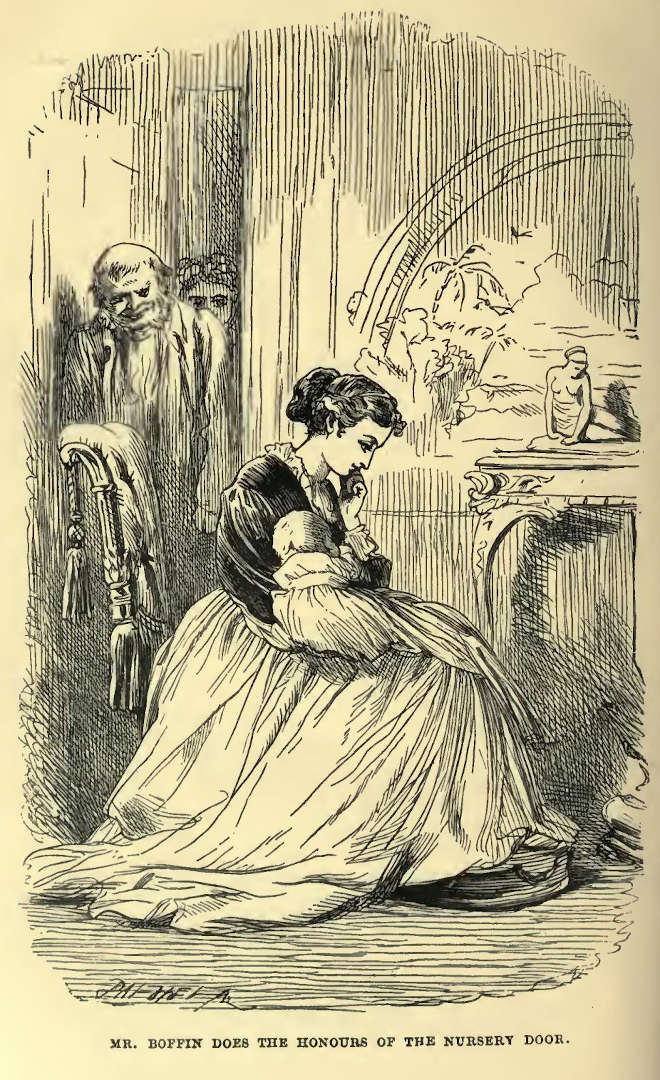
\includegraphics[scale=2.3]{04-13-01}

Then, said John Harmon, would Mrs John Harmon come and see her house?
And a dainty house it was, and a tastefully beautiful; and they went
through it in procession; the Inexhaustible on Mrs Boffin’s bosom (still
staring) occupying the middle station, and Mr Boffin bringing up the
rear. And on Bella’s exquisite toilette table was an ivory casket, and
in the casket were jewels the like of which she had never dreamed of,
and aloft on an upper floor was a nursery garnished as with rainbows;
‘though we were hard put to it,’ said John Harmon, ‘to get it done in so
short a time.’

The house inspected, emissaries removed the Inexhaustible, who was
shortly afterwards heard screaming among the rainbows; whereupon Bella
withdrew herself from the presence and knowledge of gemplemorums, and
the screaming ceased, and smiling Peace associated herself with that
young olive branch.

‘Come and look in, Noddy!’ said Mrs Boffin to Mr Boffin.

Mr Boffin, submitting to be led on tiptoe to the nursery door, looked in
with immense satisfaction, although there was nothing to see but Bella
in a musing state of happiness, seated in a little low chair upon the
hearth, with her child in her fair young arms, and her soft eyelashes
shading her eyes from the fire.

‘It looks as if the old man’s spirit had found rest at last; don’t it?’
said Mrs Boffin.

‘Yes, old lady.’

‘And as if his money had turned bright again, after a long long rust in
the dark, and was at last a beginning to sparkle in the sunlight?’

‘Yes, old lady.’

‘And it makes a pretty and a promising picter; don’t it?’

‘Yes, old lady.’

But, aware at the instant of a fine opening for a point, Mr Boffin
quenched that observation in this--delivered in the grisliest growling
of the regular brown bear. ‘A pretty and a hopeful picter? Mew,
Quack quack, Bow-wow!’ And then trotted silently downstairs, with his
shoulders in a state of the liveliest commotion.



